\chapter{Data Analysis and Results}
\label{chapter:Analysis}

In section \ref{usecases} we listed the energy efficiency use cases. In chapter \ref{chapter:background} we explained the relevance of these use case with energy efficiency and also introduced and explained the basic concepts of suitable statistical and advance analytics techniques to extract insights from data for these use cases. In \ref{chapter:platform} we explained the implementation of a model big data platform for providing an environment to perform these analysis. In this chapter we shall try to explain how we performed our data analysis using the knowledge and capabilities we developed through our work explained in previous chapters. We shall also present our results along with the critical analysis for their respective use to improve energy efficiency. Before we go into details of the use cases, analysis and results it is important that we explain the data sets.

\section{Data sets}
In our analysis we shall be using two distinct data sets provided by VTT. Both the data sets are collected by specialized devices installed on test sites as part of the Green Campus initiative. The description of data sets are as follows.

\subsection{Data set 1: Hourly energy consumption data}
This data set contains hourly readings of the energy consumption taken by specialized meters installed by VTT (Technical Research Centre of Finland) on 40 different test sites in cities of Espoo and Helsinki. Each site has at least one or more meters installed. Each installed meter on a particular site can record a particular type of energy feature consumption on hourly basis. In some cases a site have more than one meter even for same energy feature. There are four energy features considered for test sites i.e. Electricity, Heating, Water and Reactive power. We shall consider only electricity and heating in the scope of this paper. Heating feature is explained in terms of electricity consumed to produce heating.  In rest of the chapter energy features will be termed as ``feature'' and each record representing hourly consumption of a feature type will be called ``observation''.
There are approximately 1.2 Million observations taken from 144 installed meters on 40 different sites for 11 months period starting from 1st January 2013 till 30th November 2013.  Each row in data represents an observation with following information in exact sequence separated by commas. 

"Device ID","Destination Address","Building Name", "Meter", "type", "date", "hour", "Consumption"

Device is a unique id for each installed device. To avoid the confusion the site will be termed as building in rest of the document, For sake of anonymity both ``Destination Addres'' and  and``Building Name'' fields are masked as BuildingXX (where XX ranges from  01 to 40). ``Meter Numbe'' shows the number of meter on same building for one or multiple meters. Type shows the feature, date is the day date in format of YYYYMMDD, hour is the hour number of the day (0 to 23) and consumption is the consumption of the feature in respective units based on features. Since only electricity and electricity consumed for heating is considered in this paper so units are Wh (Watt hour).
To fix the scale of consumption to Kilo Watt Hour, each consumption value should be divided by 100. 

The data set is not consistent and has unequal number of observations for some building per energy type per day . Figure~\ref{fig:incon} illustrates the summary of data set and shows the inconsistencies. From figure we can see that number of records for each building are not equal. In an ideal consistent data they should be same. The inconsistency can be because of the multiple number of devices collecting data, However exploratory analysis reveal that for some buildings values were totally missing. In some cases the all the days in 11 months were not acconted for or in same cases all the hours of the day were not recorded.

\begin{figure}[!ht]
    \begin{center}
      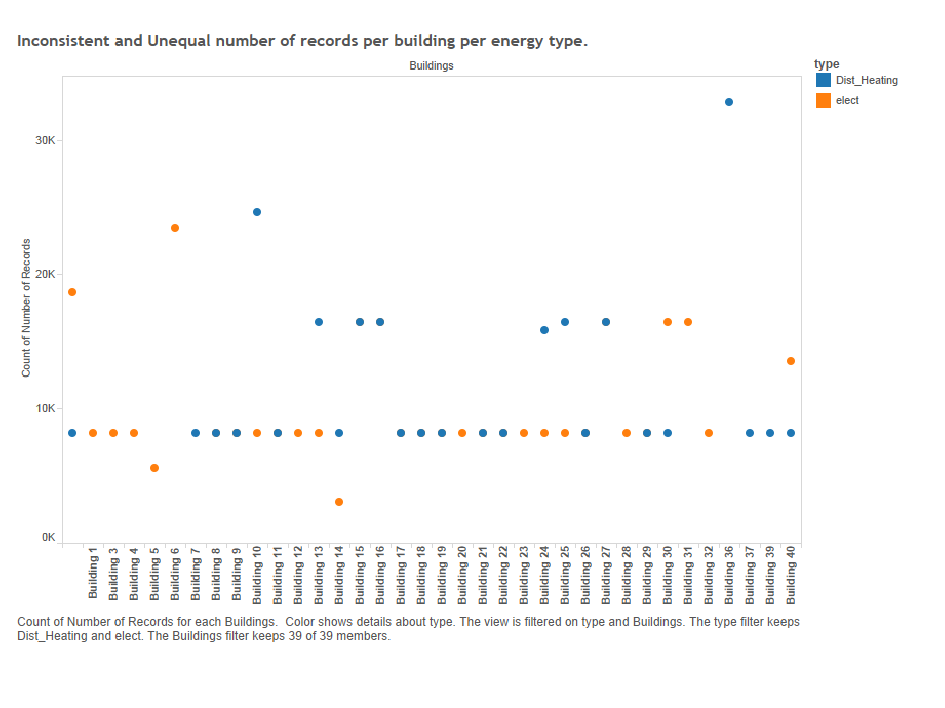
\includegraphics[width=\textwidth]{images/incon.pdf}
      \caption{Data Inconsistencies in hourly energy consumption data.}
      \label{fig:incon}
    \end{center}
  \end{figure} 
Apart from the inconsistencies shown by number of records, some building names and addresses were also missing. To handle inconsistent data, we had to adapt our analysis using aggregation techniques like averaging. We shall also explain other data cleaning and pre-processing techniques in section preprocessing of data. The implementation level details of data are available in Appendix \ref{chapter:appendixc}

To support this data set for analysis we also collected Real Estate data that include floor area of each building included in data set one. The Real Estate data was collected using following Espoo city information website.
\url{http://https://arska.espoo.fi/}


\subsection{Data set 2: Device level data} \label{nialmset}
This data set contains device level consumption of electricity collected from a residential apartment included as a test site for VTT's Green Campus initiative. The device level means that electricity  consumption  was collected for various home appliances used in that apartment. These appliances were differentiated on basis of their respective electric signal thumbprint using NIALM metering devices described in section \ref{greencamp}. The data was collected from 1st May 2013 to 30 th April 2014 in form of a text file from a VTT web service. The different fields in the data were separated by ``;''. The data set have following fields.

"Device";"Timestamp";"Consumption(Wh)"

Device field was a label for the respective home appliance e.g. Refrigerator, Freezer, TV, and Stove etc. Time stamp conains the date, hour, minutes and seconds of the recorded in  YYYY-MM-DD HH:MM:SS format. The Consumption\((Wh)\) field contains the value of electricity consumed and recorded at the instance of time. The devices that are used on demand for example TV, stove, coffee maker etc records the consumption values right after at the end of the use. For continuously used devices like refrigerator and freezer etc. NIALM devices has their inbuilt mechanism to keep recording the data. For our research we take the data record as it appears in the data set.   

\section{Use Case Categories}

As listed previously in section \ref{usecases} of this document, Following are the main use cases for our research.

\textbf{Use Case 1:} Understanding the seasonal energy usage patterns and its sensitivity with outside temperature.

\textbf{Use Case 2:}Understanding characteristics of building using daily energy consumption pattern.

\textbf{Use Case 3:}Calculate the base load of the building to identify non user consumption of buildings

\textbf{Use Case 4:}Classify building on basis of energy efficiency and analyse seasonal shifts in this classification.

\textbf{Use Case 5:} Predict daily energy consumption of various house hold devices on basis of previous consumption pattern.

Data set 1 was used for use cases 1,2,3 and 4 while data set 2 was used only for use case 5. In the similar way we grouped the use cases into two categories for analysis. Use case 1 to 4 were referred to as ``Energy Consumption patterns and classification of buildings on basis of energy efficiency''. While use case 4 was labelled as ``Prediction model for forecasting energy consumption of household devices ''


\section{Energy Consumption patterns and classification of buildings on basis of energy efficiency}
In section \ref{ecoeff} we discussed the concept of energy efficiency in context of the ecological factors. In section \ref{seasonal} we discussed the impact of outside temperature on energy usage. Similarly we established the relationship between daily load, based load and energy efficiency in setcion \ref{daily}. Now using all these concepts together we shall try to analyse our data set 1 and try to detect the daily and seasonal trends of electricity usage in green campus imitative  test buildings. We shall also try to find out the base loads for the building to see which building is consuming more energy during the off peak hours when users are not present in the building. Finally we shall try to classify the building on basis of energy efficiency a per section \ref{classify}. Following subsections will describe the each step along with explanation of the analysis and results.
\subsection{Data cleaning and pre-processing} \label{cleaning}
For preparing a tidy data set for analysis following steps were performed
\begin{enumerate}
\item Analysis was intended to be performed only for electricity and heating features so the relevant observations were extracted from the data. In rest of the document we shall consider these extracted observations only.
\item To check the consistency and quality of data in terms of number of observation per building per month per day, a quick statistical analysis was performed. Result of the analysis is illustrated in figure~\ref{fig:incon}.
\item The consumption scale was set to KWh (Kilo Watt Hour) by dividing consumption value of each observation by 100.
\item For each feature the distinct building were listed to see how many building has which type of feature available. The result shown that 32 out 40 building has observations available for electricity while 24 has observation for heating. In both the cases there were observation with null ``Destination Address'' and ``Building Name'' fields. Such observations were updated with ``Unknown'' for the respective fields. This step was particularly useful for clustering and classification part of analysis.
\item There were some other pre processing steps that are explained with their respective use cases.
\end{enumerate}

\subsection{Seasonal variation in energy consumption}
Seasonal variation in use of electricity is a very obvious phenomenon. However the important aspect for our analysis was to first see the sensitivity of energy usage with change in outside temperature as per use case 1 and then see the impact of seasonality on classification of building on basis of energy efficiency i.e. to check if a building of particular class shift to another class with change in temperature. This provides basis for use case 4. Since all of the test building are in cities of Helsinki and Espoo which are geological located close to each other so it can be safely assumed that both city has similar temperatures throughout the year. The upper graphs in figure~\ref{fig:season} shows the aggregated consumption values in a time series for all the buildings represented by two lines representing electricity and electricity used for heating respectively. While the lower graph shows the average temperature of Helsinki and Espoo during the same time of the year. The temperature data was collected using Finnish Meteorological Institutes's data API.       
 
\begin{figure}[!ht]
    \begin{center}
      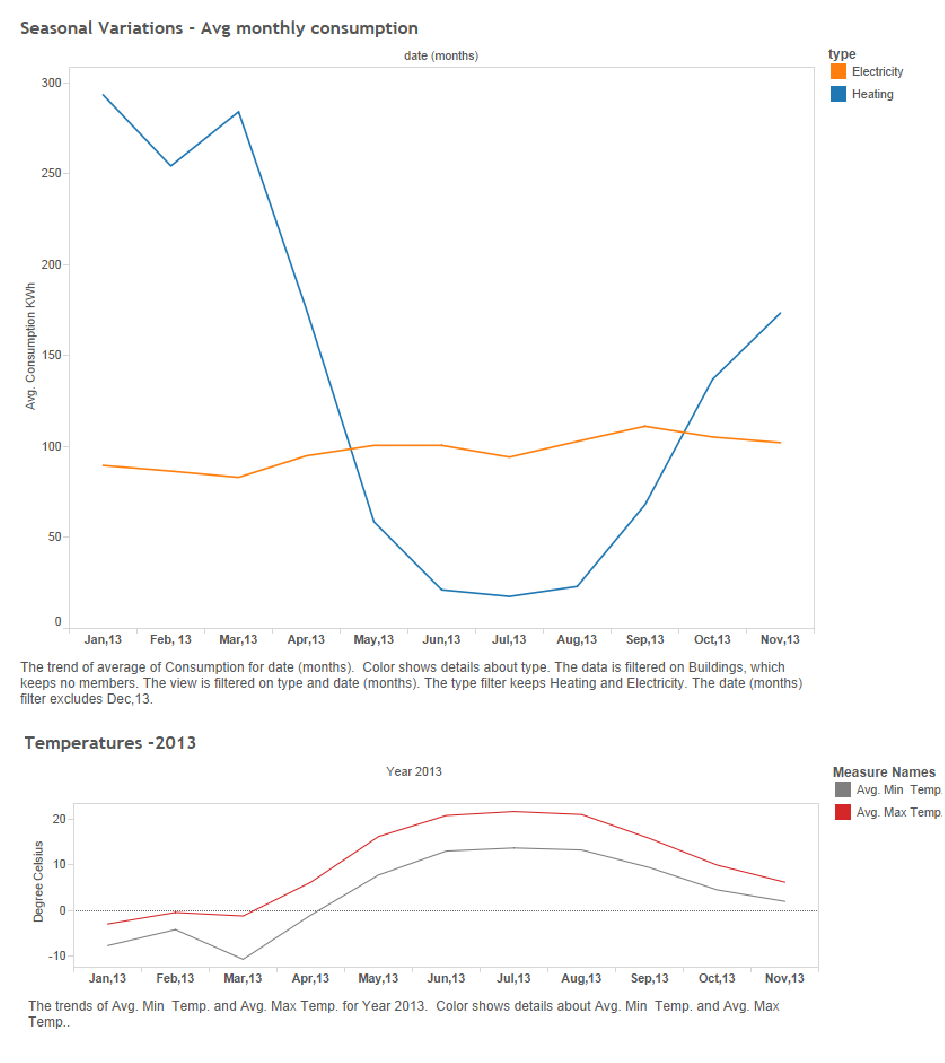
\includegraphics[scale = 0.7]{images/season.pdf}
      \caption{Seasonal patterns in usage of electricity and electricity used for heating .}
      \label{fig:season}
    \end{center}
  \end{figure} 

Figure ~\ref{fig:season} shows that electricity used for heating is more sensitive to temperatures than electricity  used for other purposes that shows a relatively stable trend through out the  eleven months period. For service providers improving heating distribution systems can contribute more to energy efficiency. 

\subsection{Daily trends}
Detecting and projecting daily trends from data set 1 can provide us two very important insights that corresponds to the use case 2 and 3. It can provide us information to suggest characteristics of a building without having any before hand information of the building. For example if the use of energy is higher during the work hours of the working days and lesser during night times and on weekends then we can suggest that the building is an office building. The second insight about the off time load or base load can refer us to the building where there can be possible electricity leakage. Rectifying such issues can improve the overall energy efficiency of the buildings.

In our analysis we detected the daily trends of the buildings by averaging the consumption of each building separately for each hour of the day. Normalizing the data for missing values was very important so instead of averaging on the total number of days for each building we took averages with the number of days for which data is available. 

\begin{figure}
        \centering
        \begin{subfigure}[b]{0.45\textwidth}
                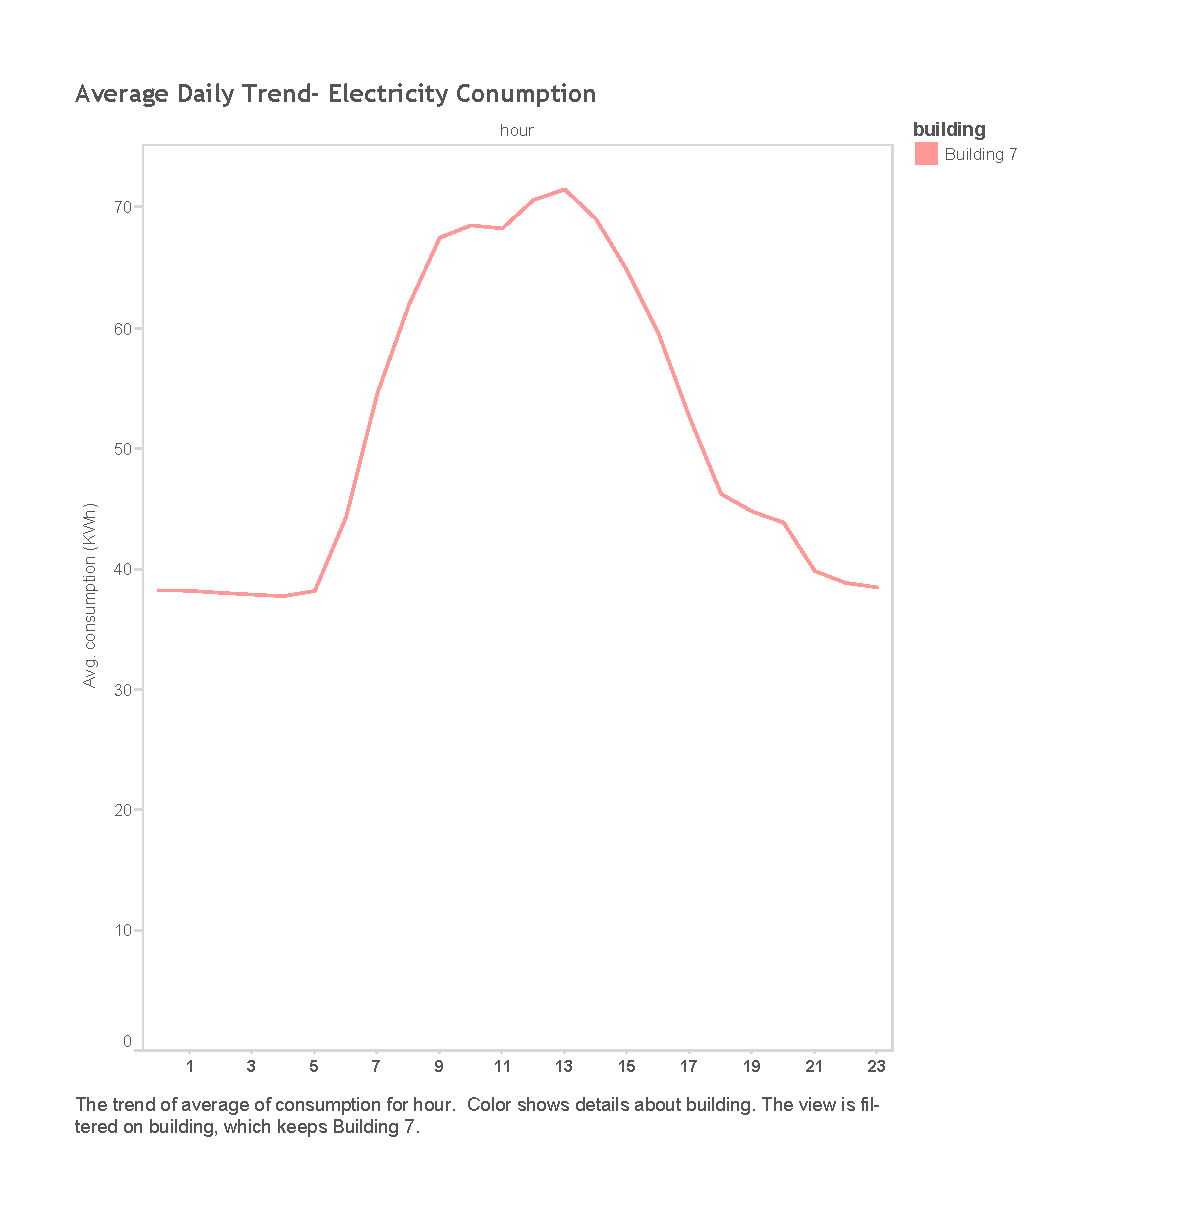
\includegraphics[width=\textwidth]{images/db6_elec.pdf}
                \caption{Building 6: Daily electricity consumption trend}
                \label{fig:elec6}
        \end{subfigure}%
        \begin{subfigure}[b]{0.45\textwidth}
                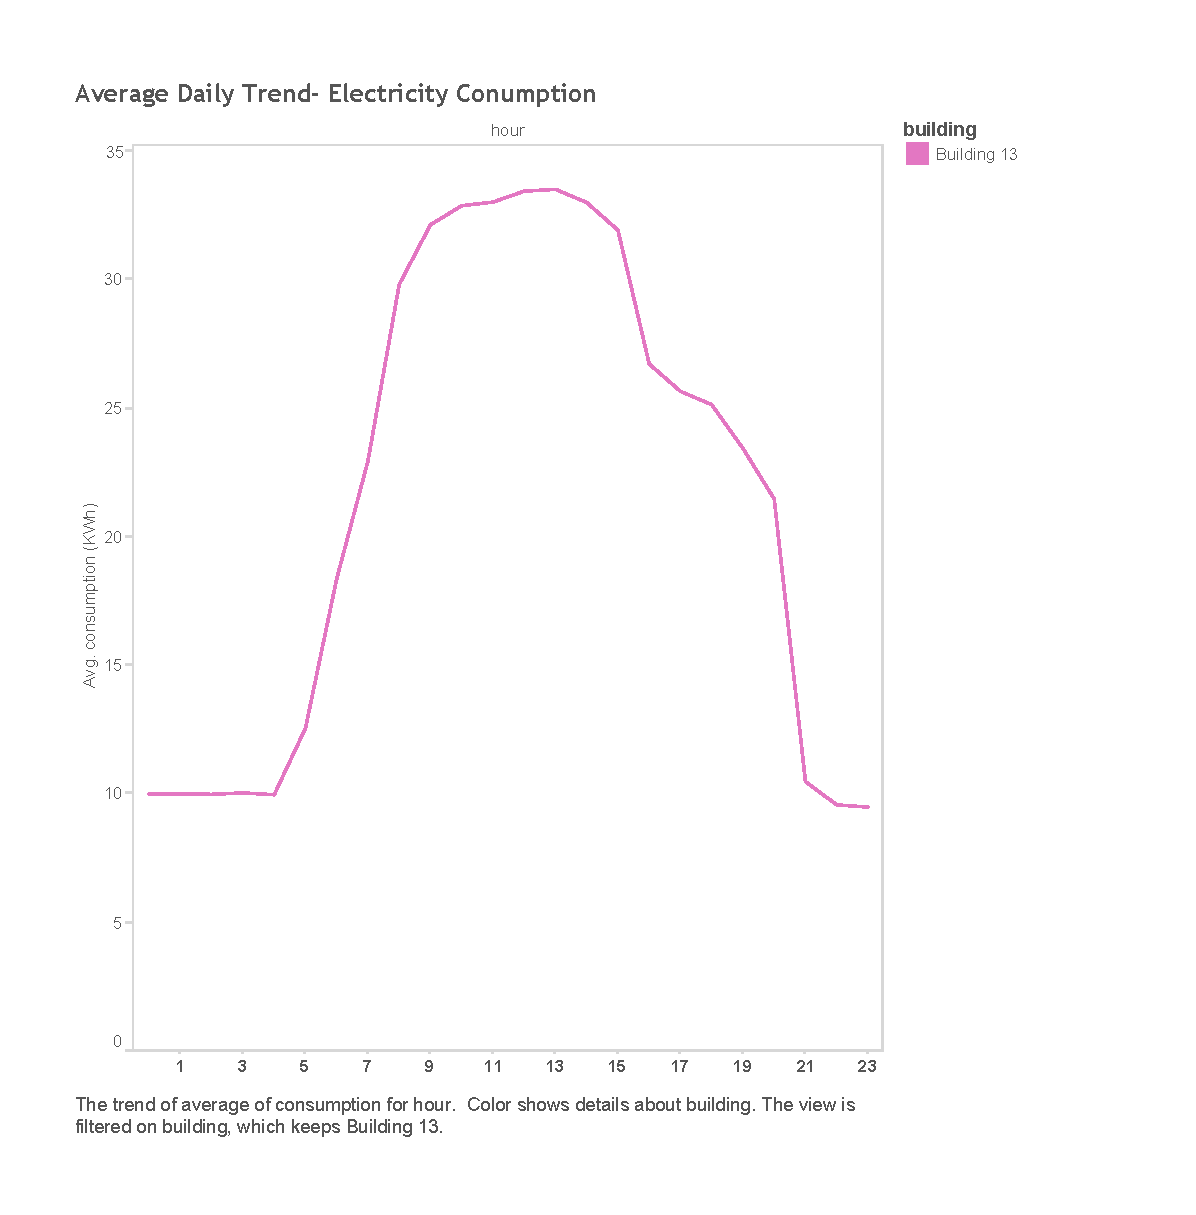
\includegraphics[width=\textwidth]{images/db13_elec.pdf}
                \caption{Building 13: Daily electricity consumption trend}
                \label{fig:elec13}
        \end{subfigure}
        
        \begin{subfigure}[b]{0.45\textwidth}
                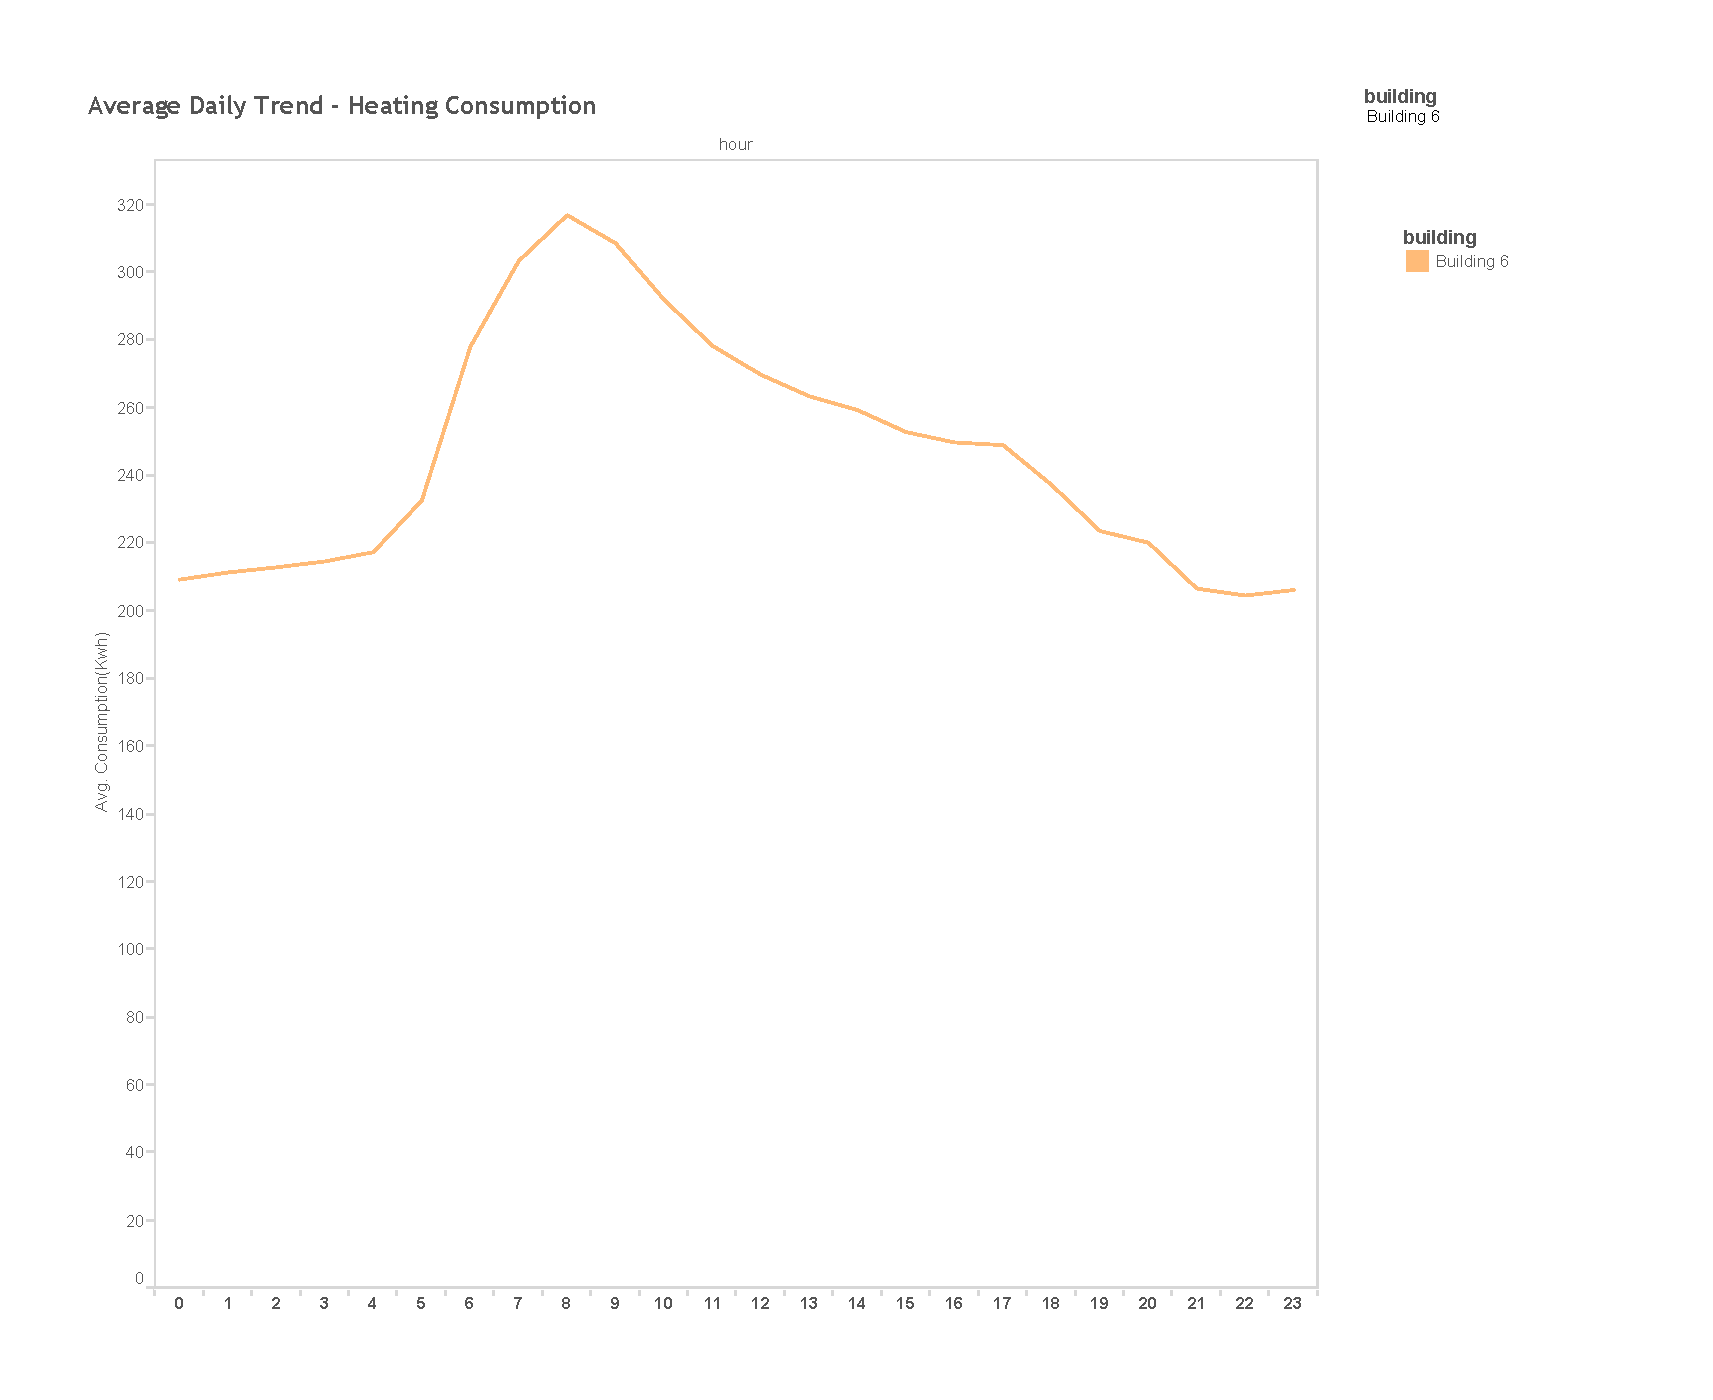
\includegraphics[width=\textwidth]{images/db6_heat}
                \caption{Building 6: Daily electricity for heating consumption trend}
                \label{fig:heat6}
        \end{subfigure}
        \begin{subfigure}[b]{0.45\textwidth}
                        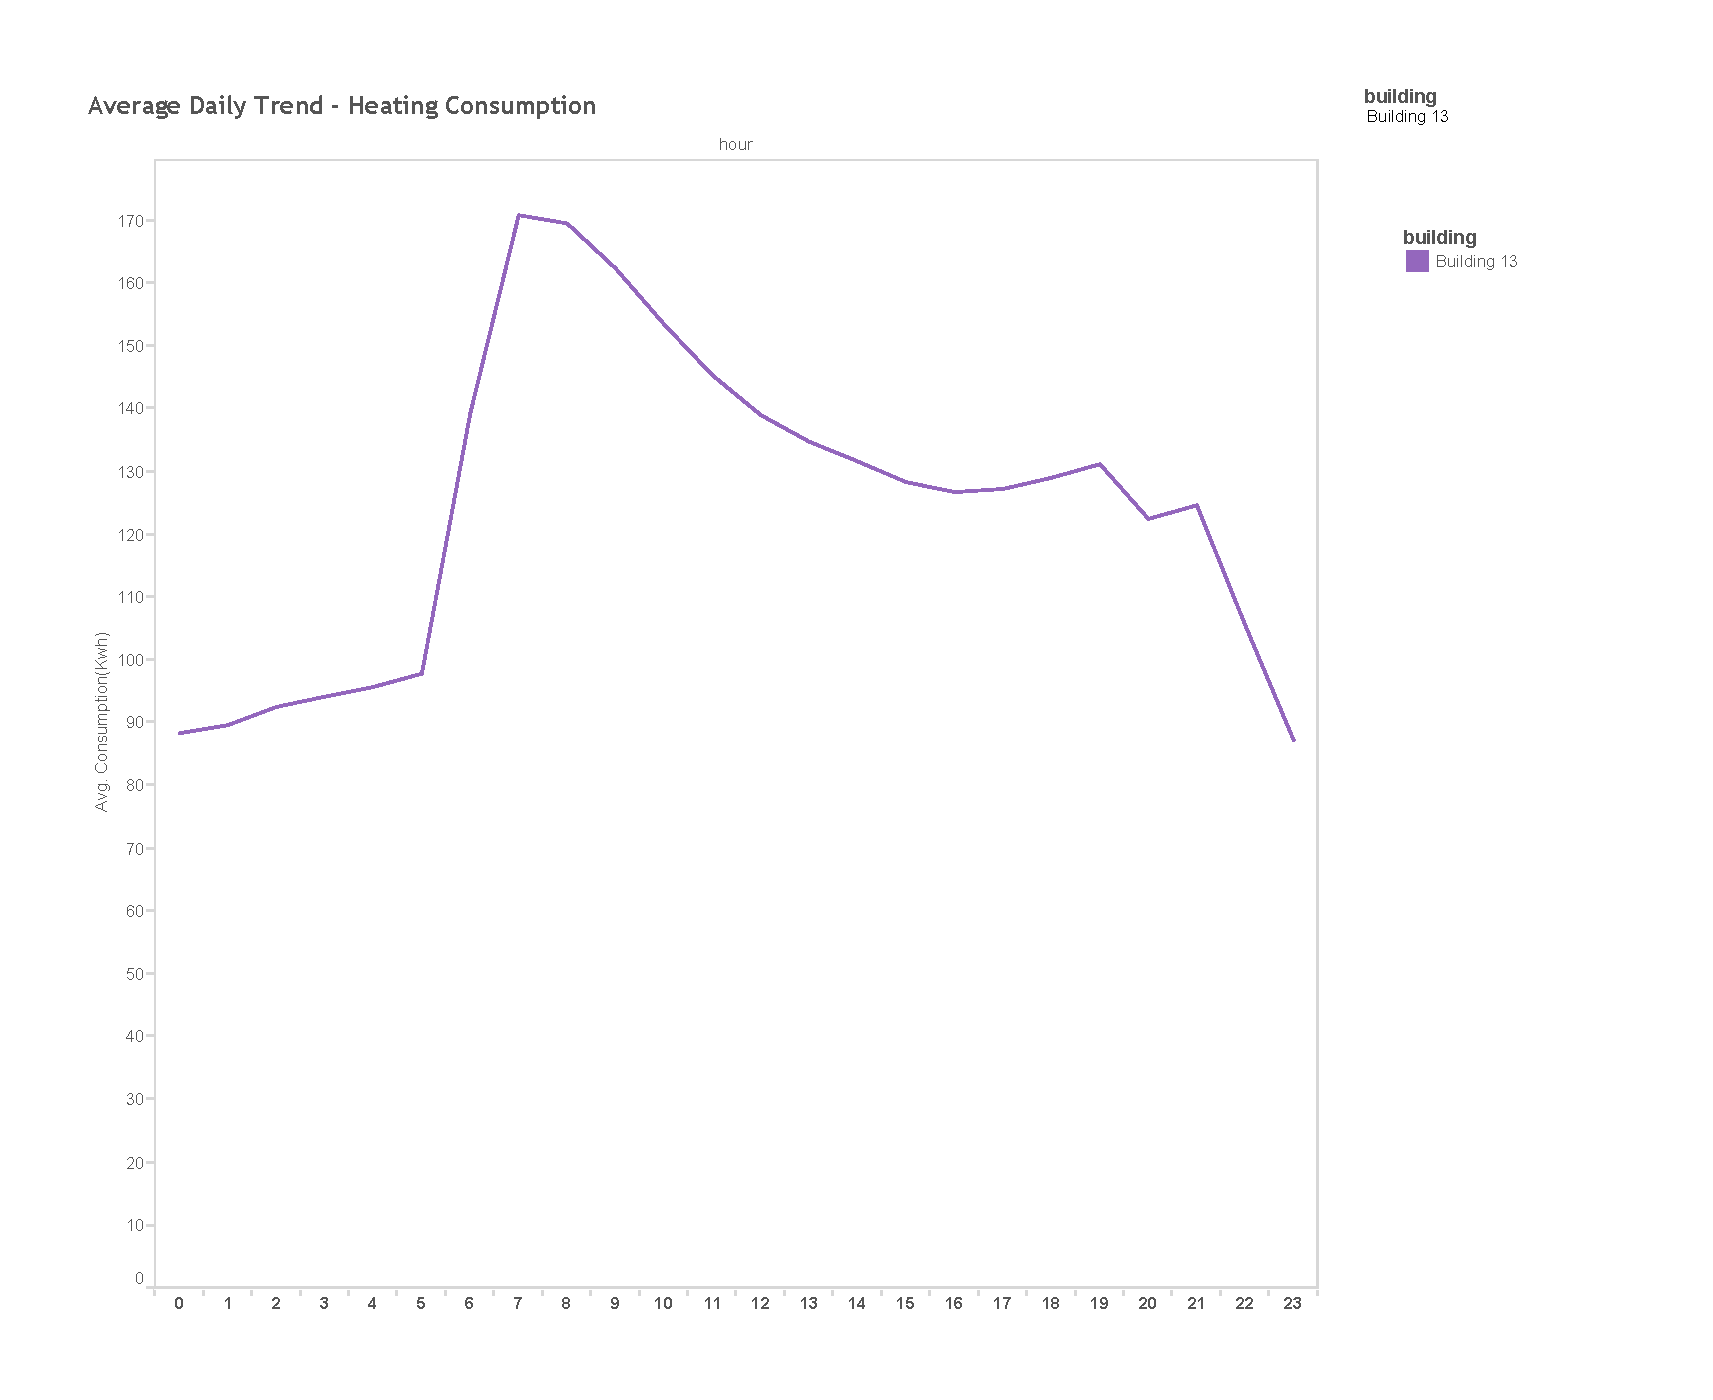
\includegraphics[width=\textwidth]{images/db13_heat}
                        \caption{Building 6: Daily electricity for heating consumption trend}
                        \label{fig:heat13}
       \end{subfigure}
     \caption{Daily energy consumption patterns}\label{fig:animals}
\end{figure}

Figures \ref{fig:elec6} and \ref{fig:elec13} shows the average daily electricity consumption of two buildings from our data i.e. Building 6 and 13 respectively. While  \ref{fig:heat6} and \ref{fig:heat13} shows the electricity consumption for heating for same buildings. Both type of consumptions are higher during office hours suggesting the purpose of building.  While each building has different base loads. Base load hours are very visible in the the daily trends graphs. An interactive dashboard is available to observe the trends for all the buildings is available on following website.

\url{http://https://arska.espoo.fi/}

A quick exploratory analysis of the trends suggests that all buildings are office buildings . Secondly the base load hours are hour 0,1,2 and 23. The base loads can then be calculated by averaging the consumption for these  hours. Appendix \ref{chapter:appendixd} contains the list of calculated base loads for each building in each month of the year within available data.

\subsection{Classification of buildings on basis of energy efficiency}
Classification on basis of energy efficiency can be used as a tool to benchmark and segregate inefficient energy consumption units from efficiently performing buildings. Such classification can narrow down the scope of research for finding the possible energy leakages and faults. We discussed the main concepts and the k-means clustering technique we used for our analysis in section \ref{classify}. The existence of some similarity is a pre condition for any cluster analysis technique. To test this on our data set we calculated average hourly energy efficiency using equation~\ref{spec_energy} for each building. Figure~\ref{fig:hr_m2} confirms the availability of similarly behaving buildings in terms of energy efficiency. 
\begin{figure}[!ht]
    \begin{center}
      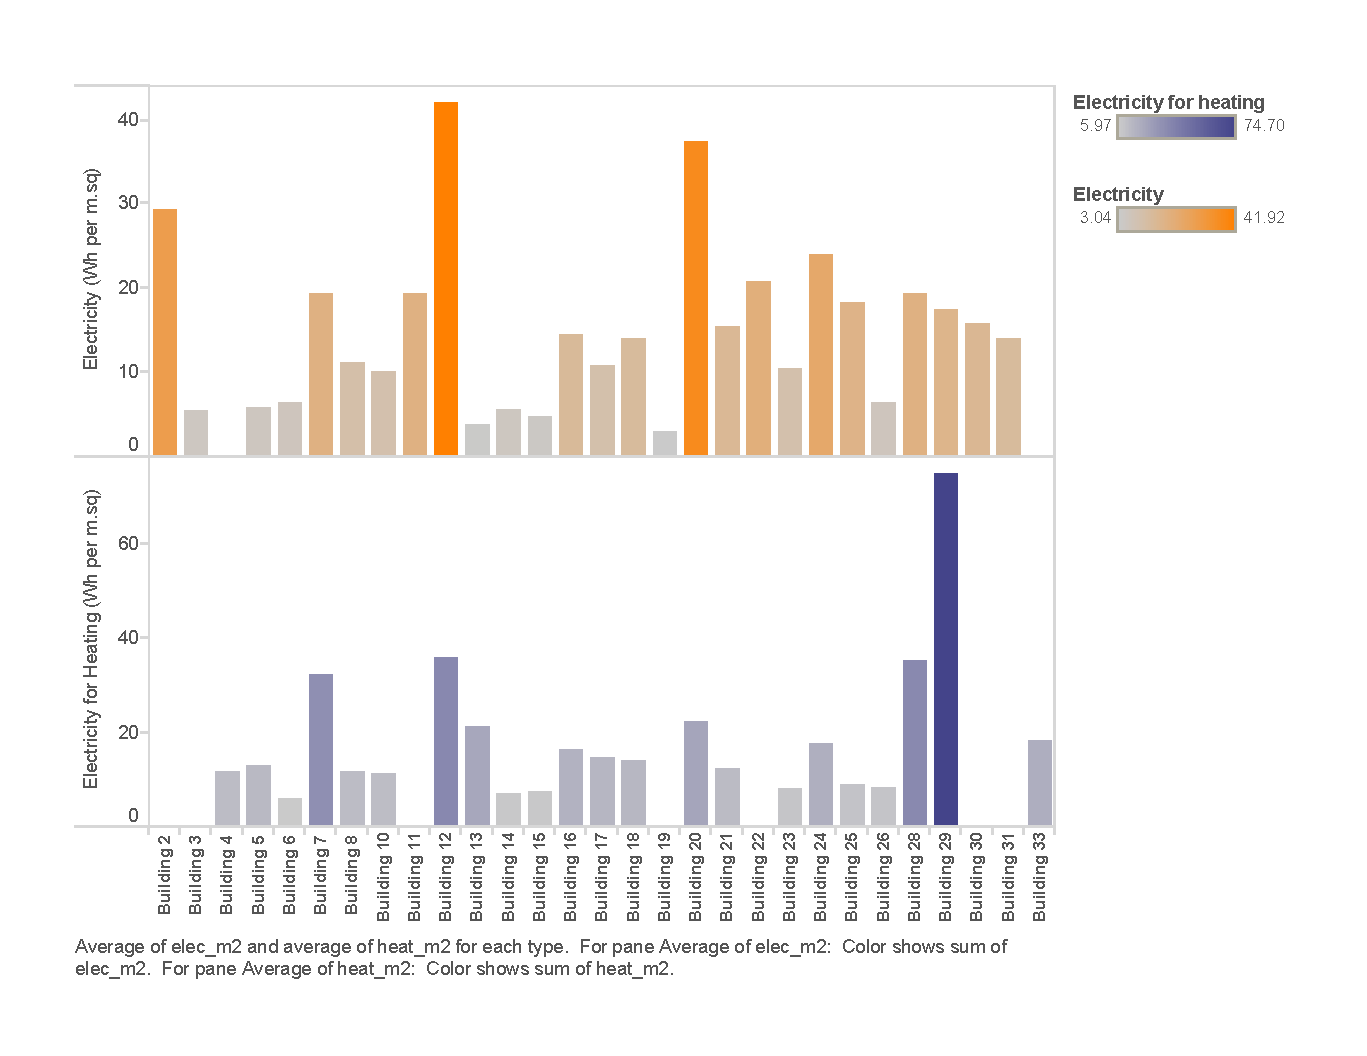
\includegraphics[scale = 0.6]{images/hr_m2.pdf}
      \caption{Energy efficiency of buildings with hourly average consumption.}
      \label{fig:hr_m2}
    \end{center}
\end{figure} 

\subsection{Data processing for cluster analysis}
K-means algorithms needs input data in form of a matrix, where the values of each feature are defined in their respective columns while each row represents a data point that will be grouped together in forms of clusters. In our case we had two energy features i.e. electricity and electricity used for heating. While average monthly energy efficiency value for each month and each building was represented by a row in input matrix. The reason for considering average monthly values for buildings was to analyse the energy efficiency of the building through out the eleven months period. So in this way our input matrix consisted of 
\begin{lstlisting}
Number of rows, i = 2
Number of columns, j = Number of buildings x 11 
\end{lstlisting}
Following are the main data processing steps that we performed on data for producing a tidy input matrix for our cluster analysis. These steps are performed on the data set that we had as output of the preliminary data pre-processing described in section \ref{cleaning}.
\begin{enumerate}
\item We segregated the electricity and electricity used for heating records from each other.
\item We calculated the average daily consumption for each building and each energy type first and then calculated the average monthly consumption in similar way. It was important to normalize the data by taking the averages on basis of number of records available for hours within a day and then days within a month. 
\item We then arranged calculated average monthly consumption values for each energy type in form of a matrix labelled with building and month names as separate columns. We called this matrix as ``energy consumption matrix''.   
\item At this stage our energy consumption matrix had few buildings for which consumption values were missing for either type of energy. We removed these building to avoid inconsistency in data for cluster analysis. 
\item We then introduced the real estate data i.e. ground floor area of the respective buildings into our energy consumption matrix. Using equation ~\ref{spec_energy}, we calculated the energy efficiency values for each energy type. We termed the resulting matrix as ``energy efficiency matrix''.
\item Till this moment we had energy efficiency in units of Kilo Watt hour per meter square. We converted the values into Watt hour per square meter. This was an optional step and it was performed just to avoid handling small decimal values.
\item To prepare the final input matrix we removed the labels and leaving two columns of energy efficiency values for two target types of energies.
\item To finalize the K-means input matrix. We used R programming \textbf{scale()} function to set the unit variance for all matrix elements. This function could have also normalized the scale of measurement, However in our case it was already a similar unit for both energy types i.e. \((Wh/m^2)\).        
\end{enumerate}
\subsection{K-means clustering analysis and results}
Our use case requirement was to classify the buildings into four categories of high efficiency, moderate efficiency, low efficiency and poor efficiency buildings. So we had the pre-defined K value of 4. We applied k-means clustering on our input matrix using R programming \textbf{kmeans()} function.

As a post processing step we combined the resulting cluster values to the energy efficiency matrix in front of their respective labels \((Building Name + Month Name)\) and energy efficiency values \((electricity and electricity used for heating)\). We termed this matrix as  ``clustered matrix'. The clustered matrix was then fed into Tableau public as a CSV file to create interactive dashboard and visualizations. Figure~\ref{fig:kmeans} visualizes the result of clustering.  

\begin{figure}[!ht]
    \begin{center}
      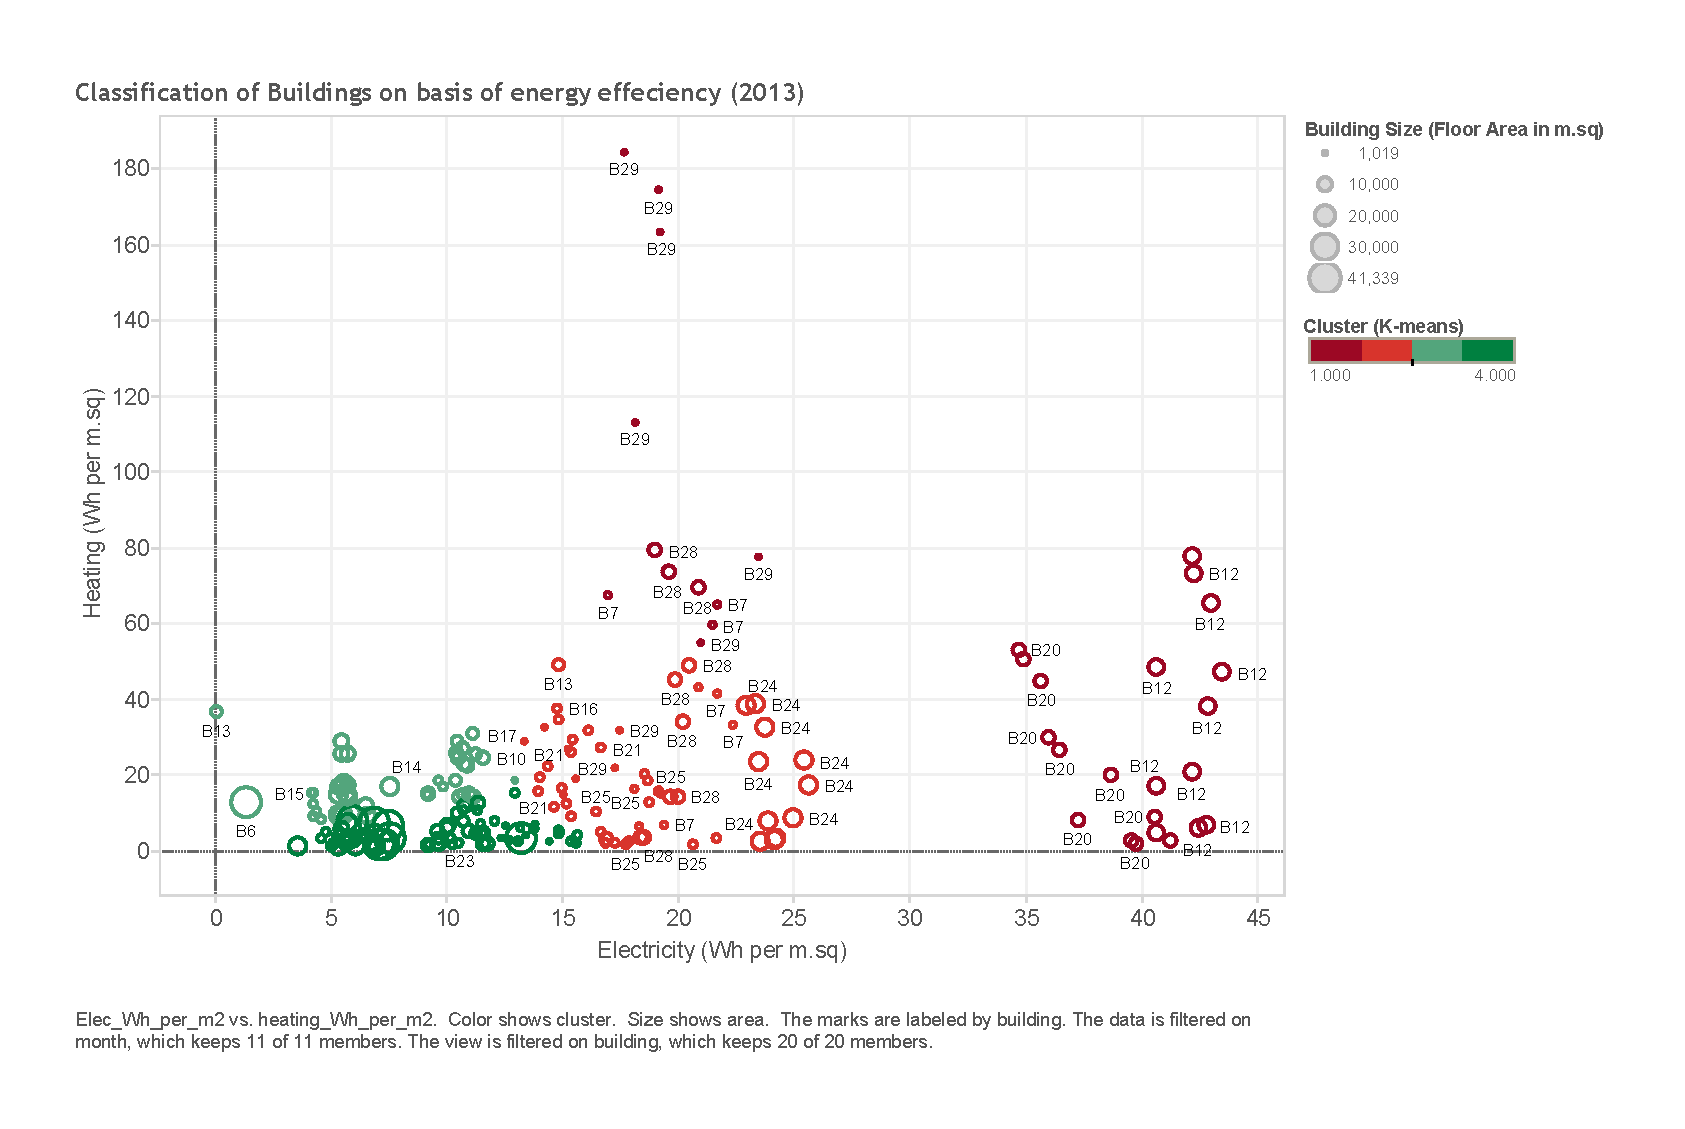
\includegraphics[width=\textwidth]{images/kmeans.pdf}
      \caption{K-means clustering, Average monthly energy efficiency per each building.}
      \label{fig:kmeans}
    \end{center}
\end{figure} 

Each bubble on the graph represents a months average energy efficiency value for a particular building. The colour of the bubble represent the respective cluster or class. While size of the bubble represents the size of the building. Cluster numbers are from 1 to 4, where 4 represents the highly efficient cluster and 1 is for the most energy inefficient cluster of the buildings. Figure ~\ref{fig:kmeans_jan} shows the one month subset of the clustered values. Each buble represent average energy effeciency in month of January. 
\begin{figure}[!ht]
    \begin{center}
      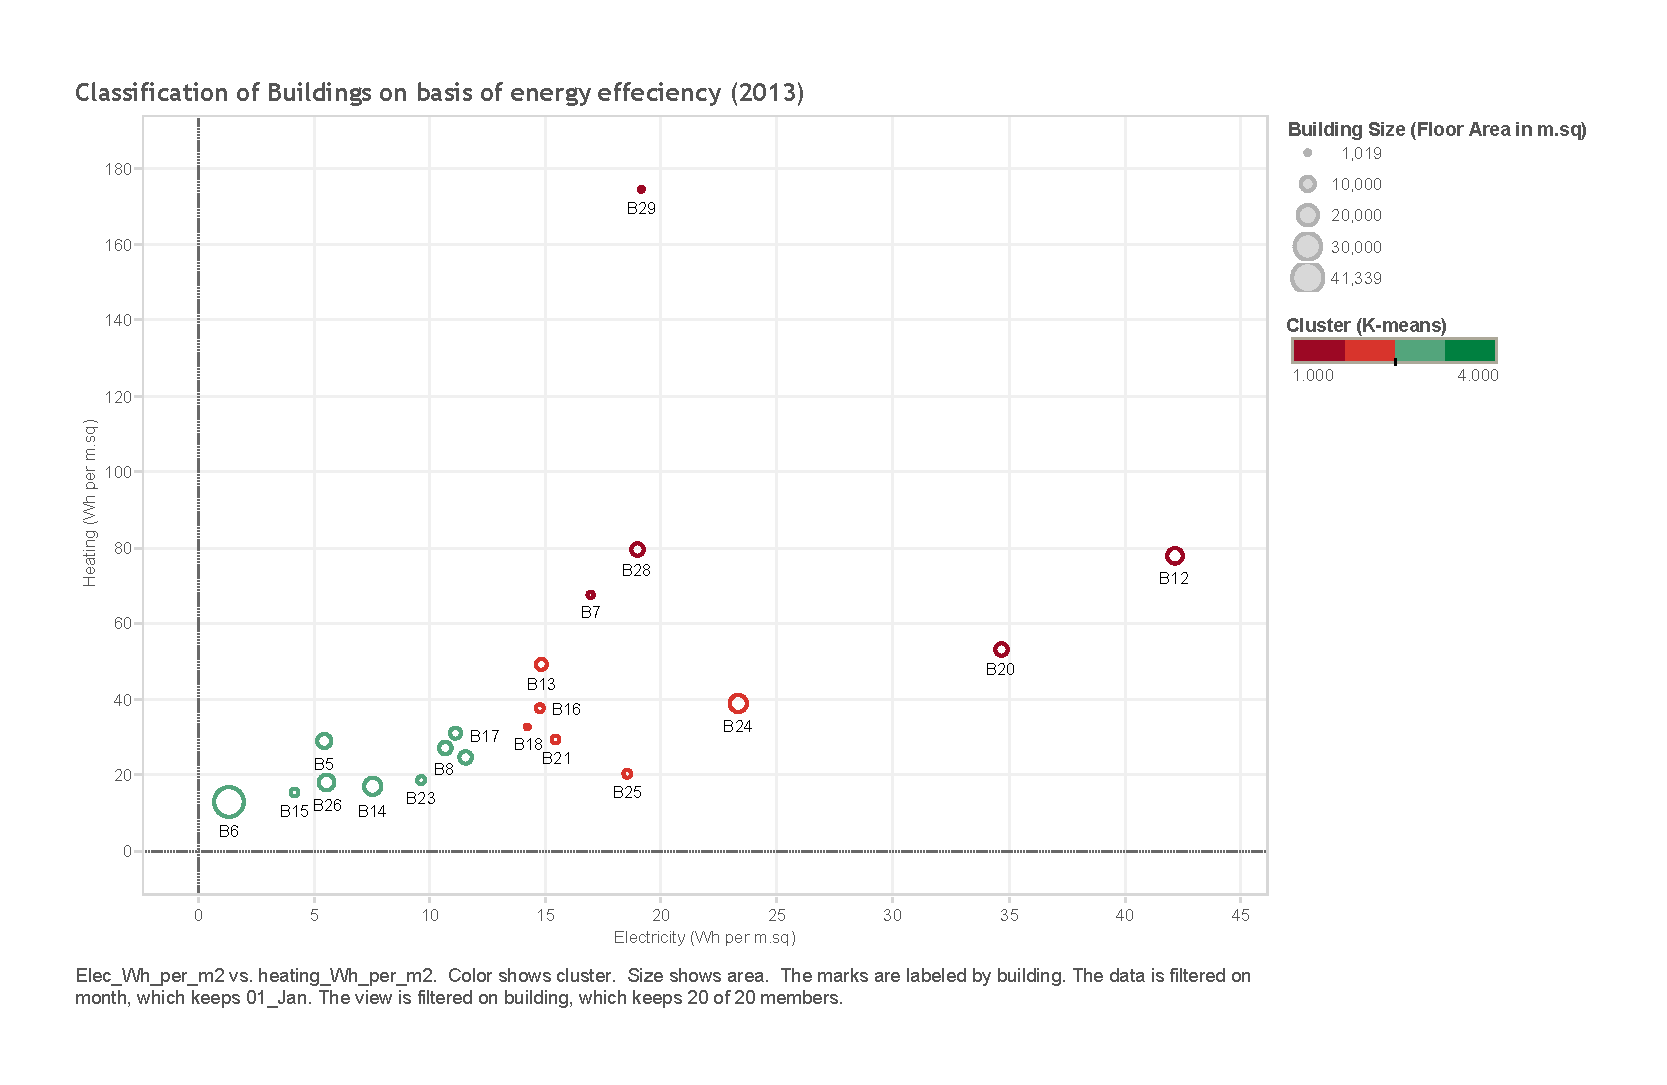
\includegraphics[width=\textwidth]{images/kmeans_jan.pdf}
      \caption{K-means clustering, One month view.}
      \label{fig:kmeans_jan}
    \end{center}
\end{figure} 

\textbf{Insight:} Figures~\ref{fig:kmeans} and ~\ref{fig:kmeans_jan} reflect a very important insight that some of the bigger size buildings are in high or moderate efficiency clusters while some of the smaller buildings are in inefficient clusters. Such extreme case can be good targets for case studies. The low efficiency buildings may have some energy leakages, faults or inefficient usage practices while the high efficiency buildings may suggest good practices for using energy. 

As part of the use case, we also studied the behaviour of buildings using same cluster analysis. Figure~\ref{fig:clustershift} illustrates the behaviour of different buildings during the 11 months period. Figuresb~\ref{fig:tri_1} and \ref{fig:tri_2} presents the behaviour of building 29 and building 7 respectively. Both the buildings shift among three different clusters. While figures \ref{fig:dbl} and \ref{fig:single} represents the buildings 16 and 24 that shows shift between two clusters and no cluster shift respectively.
\\
\textbf{Insight} Figure ~\ref{fig:clustershift} shows the fact that buildings are not equally energy efficient or inefficient through out the year. 

An interactive dashboard is available for viewing the behaviour of all the buildings in 11 months of data via following web address undera classification tab.

\url{http://catalyc.net/}
   

\begin{figure}
        \centering
        \begin{subfigure}[b]{0.45\textwidth}
                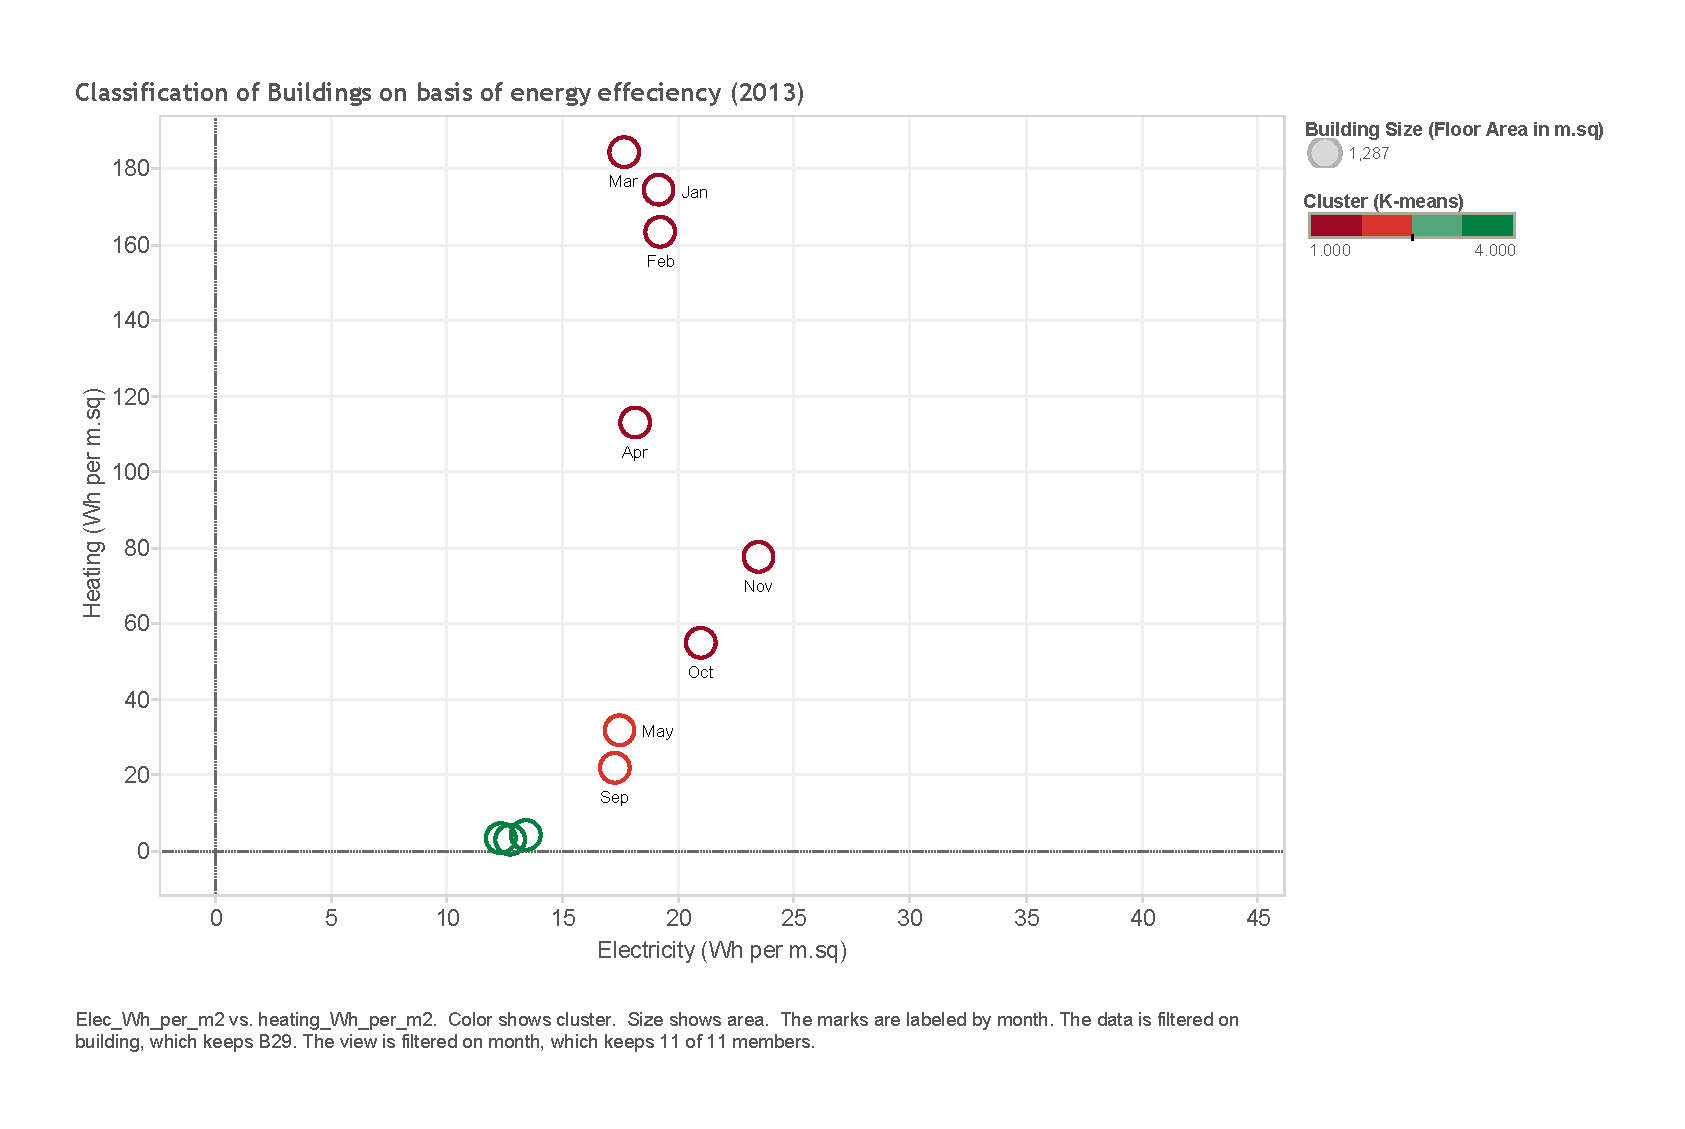
\includegraphics[width=\textwidth]{images/kmeans_b29_3c.pdf}
                \caption{Building 29:  Triple shift}
                \label{fig:tri_1}
        \end{subfigure}%
        \begin{subfigure}[b]{0.45\textwidth}
                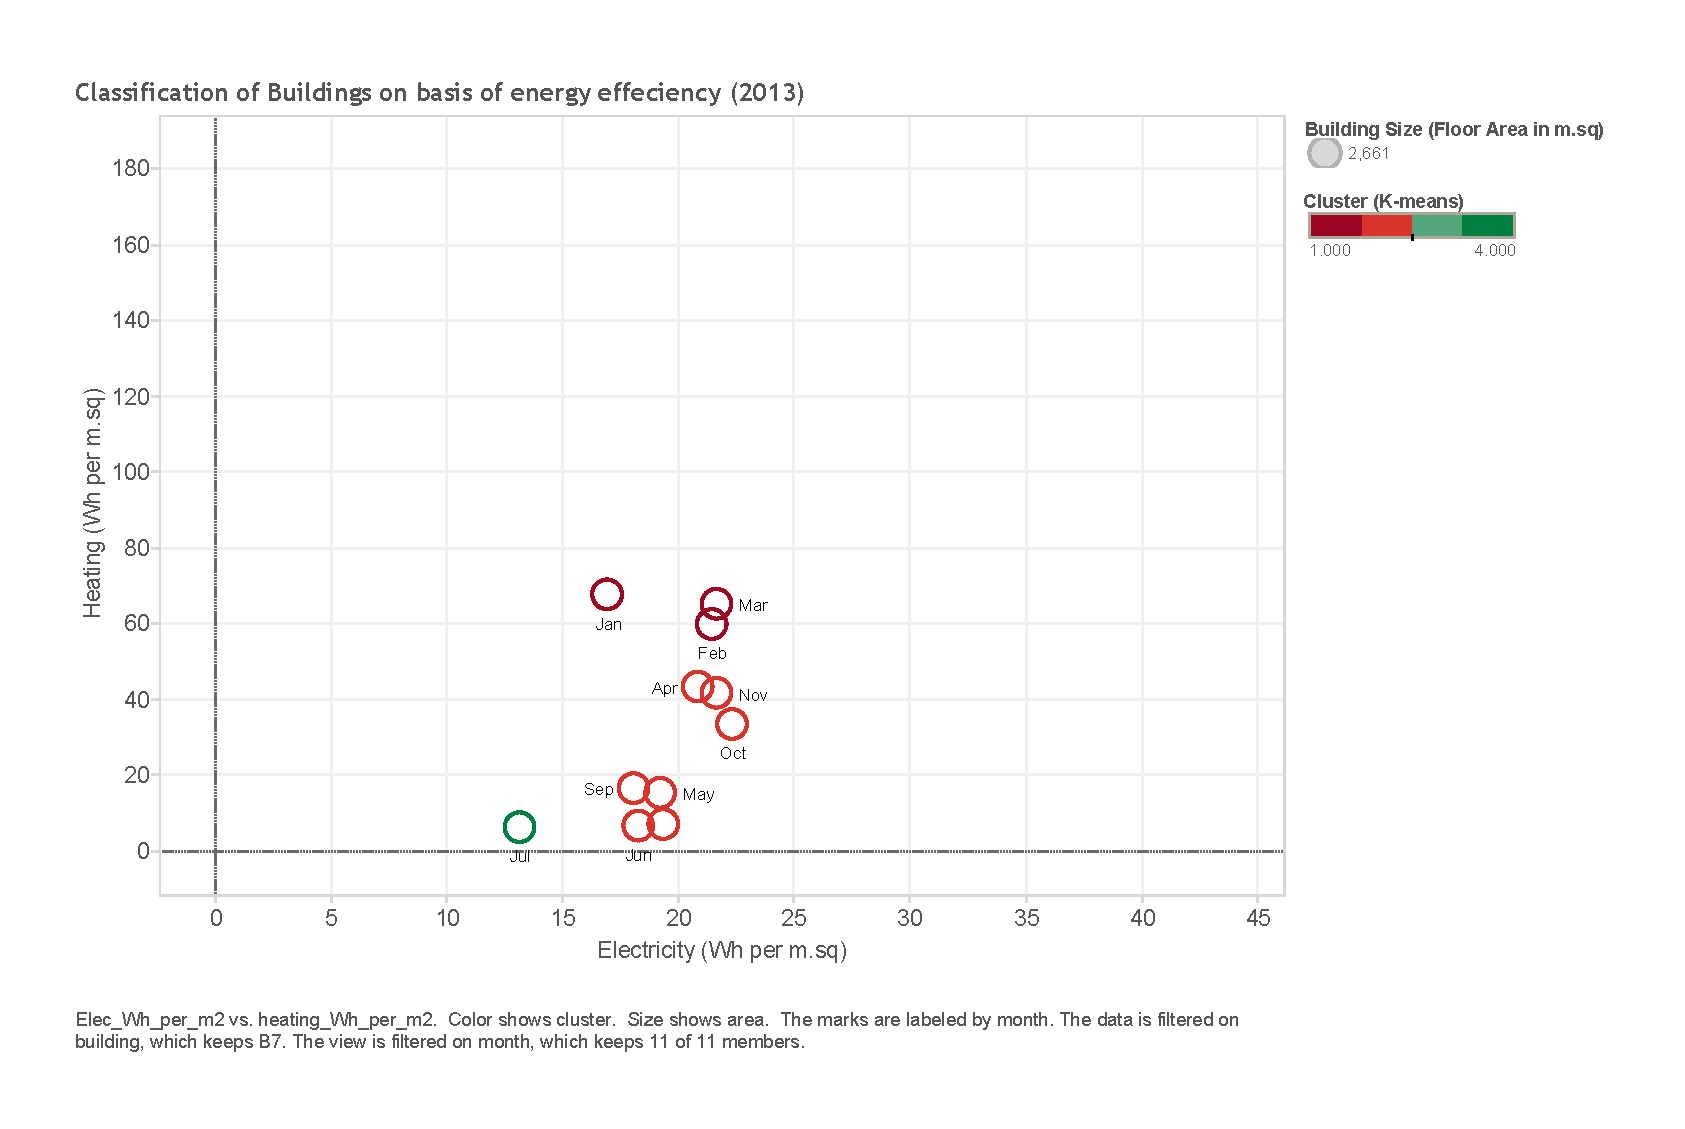
\includegraphics[width=\textwidth]{images/kmeans_b7.pdf}
                \caption{Building 7: Triple shift}
                \label{fig:tri_2}
        \end{subfigure}
        
        \begin{subfigure}[b]{0.45\textwidth}
                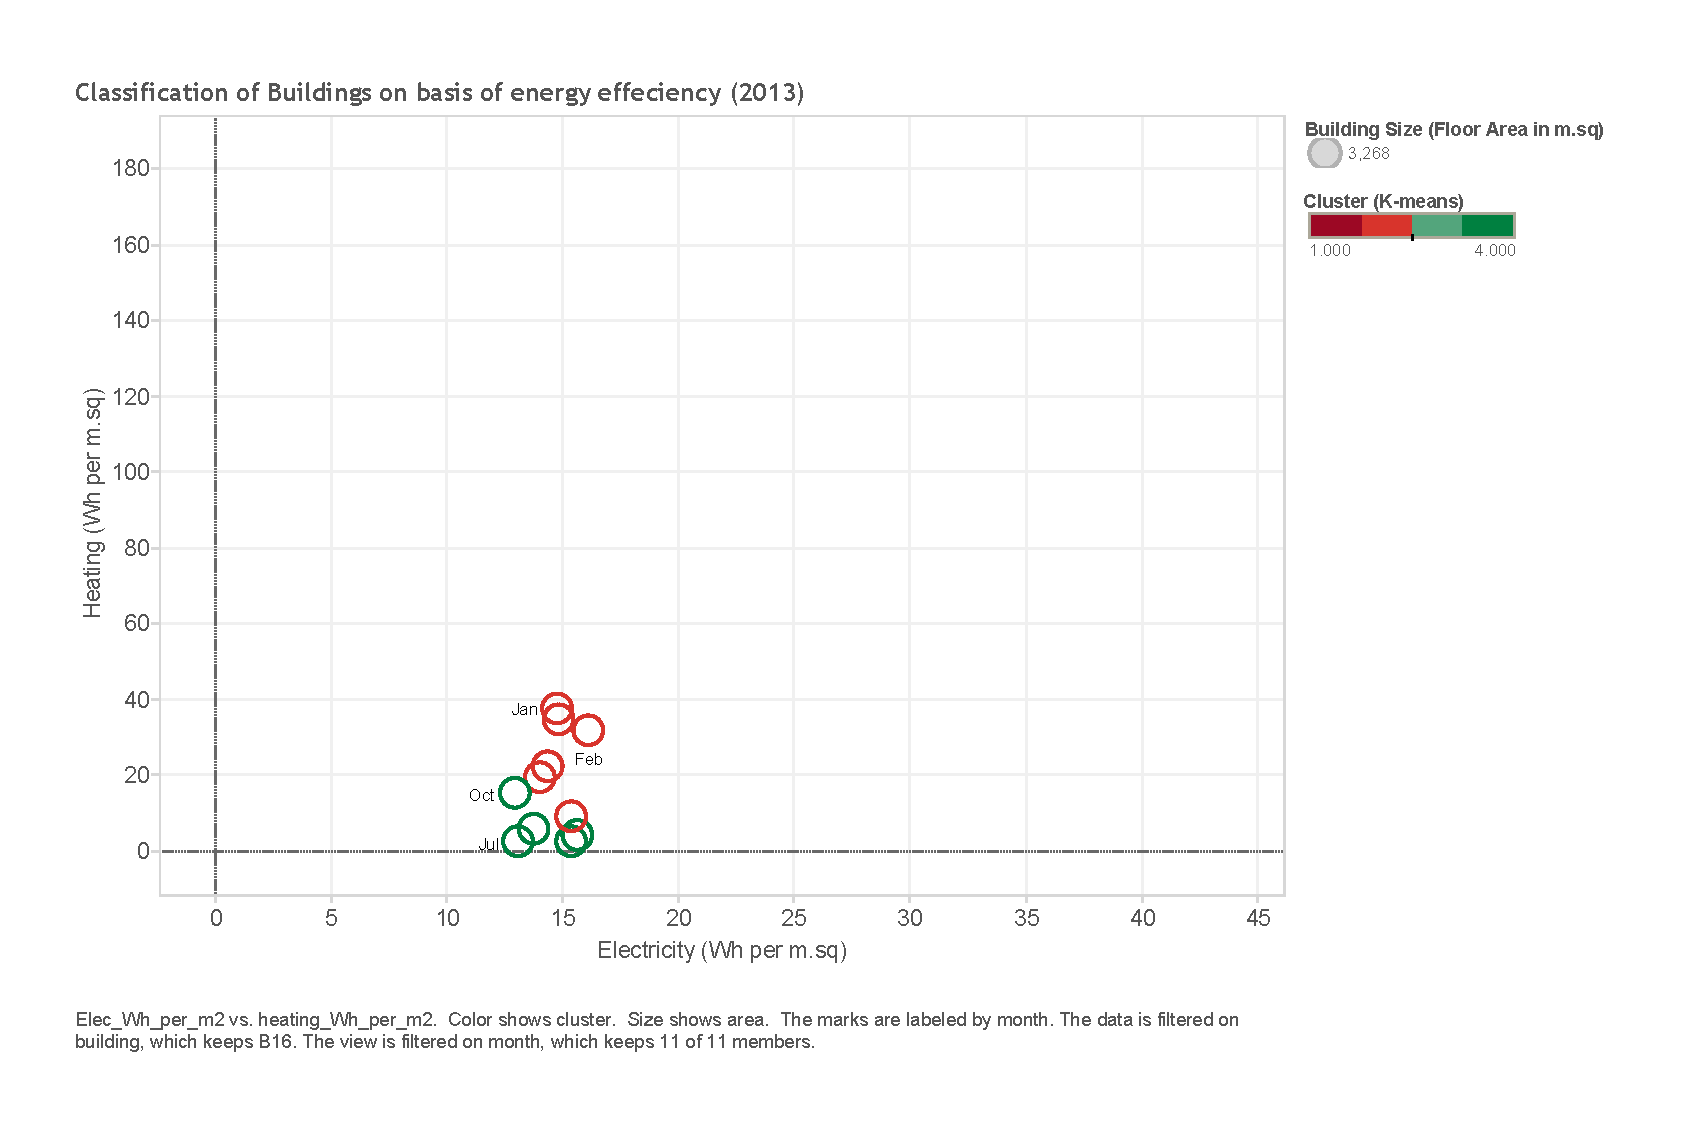
\includegraphics[width=\textwidth]{images/kmeans_B16_2c.pdf}
                \caption{Building 16: Double shift}
                \label{fig:dbl}
        \end{subfigure}
        \begin{subfigure}[b]{0.45\textwidth}
                        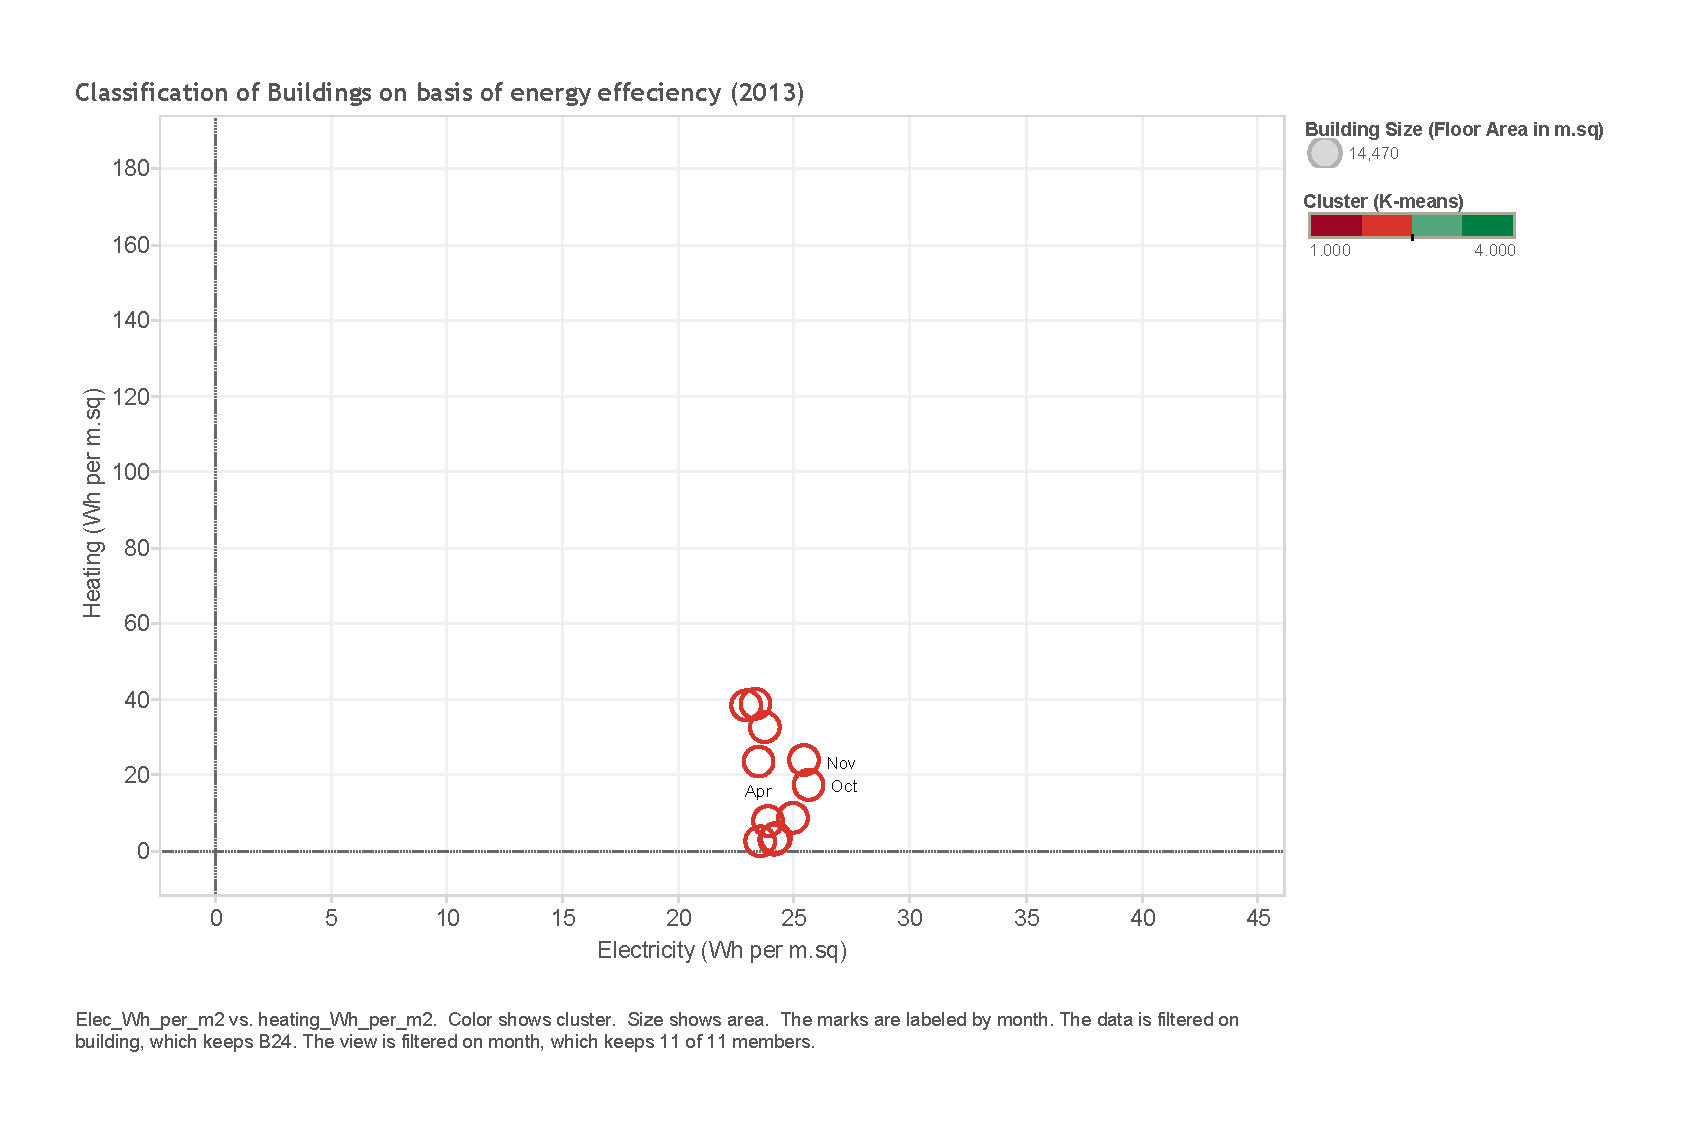
\includegraphics[width=\textwidth]{images/kmeans_b24_no.pdf}
                        \caption{Building 24: No Shift}
                        \label{fig:single}
       \end{subfigure}
     \caption{Energy effeciency cluster shift during 11 months}\label{fig:clustershift}
\end{figure}

\section{Prediction model for forecasting energy consumption of household devices}
We discussed the data set collected by NIALM devices in section \ref{nialmset}. Using this data set we tried to implement a limited prediction model to forecast the usage of household appliances. There were nine different appliances included in our data set i.e. Refrigerator, Freezer, Dishwasher, Laundry machine, Coffee maker, Stove, TV or PC, and Microwave oven. Some of the devices are generally in continuous use e.g. freezer and refrigerator. While others are use on need basis e.g. stove, coffee maker, laundry machine etc. Even in such devices, frequency of usage can be different e.g. stove, coffee maker etc are usually used on daily basis while laundry machine can be used once in a week. The limited scope of our prediction model means that we are not dealing with all this diversity. Instead we forecast only for those devices which are in continuous usage e.g. freezer and refrigerator.      

    